\section{Andmebaasi projekteerimine}
\label{chapters:analysis_database}
Arendatavas infosüsteemis kasutatakse relatsioonilist andmebaasi, mille puhul andmeb on koondatud
tabelitesse. 
Andmebaasi primaarvõtmeteks kasutatakse GUID võtmed, mis on 128-biti pikkusega sõne.
GUID on piisavalt pikk, et võtme unikaalsus oleks piisava tõenäosusega tagatud. Samuti GUID on genereeritud
raamistikuga, mis on kiirem \cite{guid_definition}. Kuna infosüsteemis on kasutusel ORM Entity Framework, 
siis andmebaasi skeemi luuakse automaatselt koodis ehitatud mudeli järgi. Vaatamata sellele, enne 
andmemudeli realiseerumist koodis peab läbi mõtlema selle ülesehitust ja loogilisi seoseid andmemudeli
objektide vahel.

Kuigi minimaalse elujõulise toote arendamise raames on otsustatud arvutusprogrammist elimineerida mittehomogeensete
(mitmest materjalist koosnevate) kihtide arvutamist, siiski tuleb sellise võimalusega arvestama tulevikus. Selle jaoks on andmemudelis 
olemas alamkihi objekt (\textit{SubLayer}). Iga konstruktsiooni kiht võib koosneda mitmest alamkihist.
Näiteks paksusega 200 mm puitsõrestik seinas 50 mm paksusega puitpostide vahel paikneb 550 mm mineraalvilla. 
Sellisel juhul oleks kihi (\textit{MainLayer}) sees oleks kaks alamkihti, üks on paksusega 50mm, mille materjaliks
on puit ning teine on paksusega 550 mm, mille materjaliks on vill. Selline struktuur võimaldab mudeldada
peaaegu kõikvõimalikud ehituses kasutusel olevad lahendused. Kuna esialgu antud funktsionaalsust
ei tehta, luuakse igakord uus kiht ühe alamkihiga. Sellisel juhul ka tulevikus süsteem toetab varem loodud
konstruktsioonide arvutamist. Kihtide mudeldamist käsitlev diagrammi osa on toodud pildil \ref{fig:db_layers_model}.

\begin{figure}[ht]
    \centering
    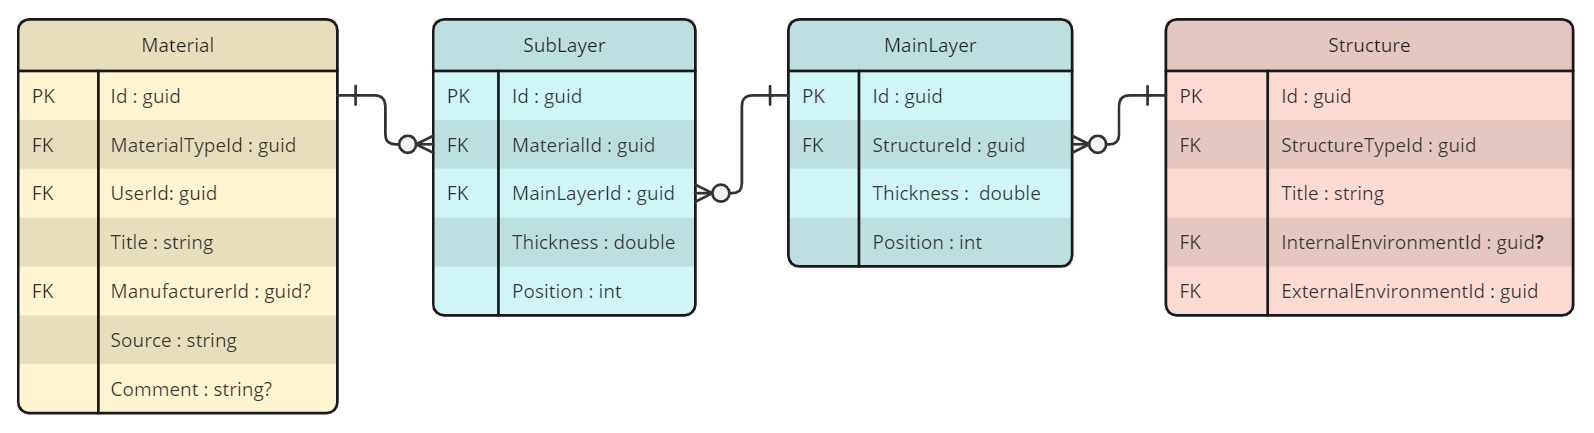
\includegraphics[width=1\textwidth]{figures/analysis/db_desing_1.png}
    \caption[Konstruktsiooni kihtide andmemudel]{\textit{Konstruktsiooni kihtide andmemudel}}
    \label{fig:db_layers_model}
\end{figure}

Selleks, et konstruktsioonide ehitusfüüsikaline arvutamine oleks võimalik, süsteemis peavad olema ka 
materjali füüsilised omadused: soojusjuhtivus ja üks veeaurujuhtivust kirjeldatavatest omadustest. On 
aga ka võimalik, et tulevikus tööriistakasti lisatakse teised arvutusprogrammid, mille jaoks on tarvis teada
teisi omadusi. Selleks, et võimaldada tulevikus luua vajadusel uusi materjalide omadusi, andmebaasimudelis
on olemas järgmised objektid: omadus (\textit{Property}) ja materjali omadus (\textit{MaterialProperty}) - pilt 
\ref{fig:db_properties_model}. Lisaks, selline mudel võimaldab säilitada omaduste muutuste ajalugu.
Selleks, et arvutused oleksid usaldusväärsed, peab igal materjali omadusel olema märge sellest, kas 
tegemist on verifitseeritud andmetega ja mis on andmete allikas (nt tootja dokumentatsioon, teadusartikkel).

\begin{figure}[ht]
    \centering
    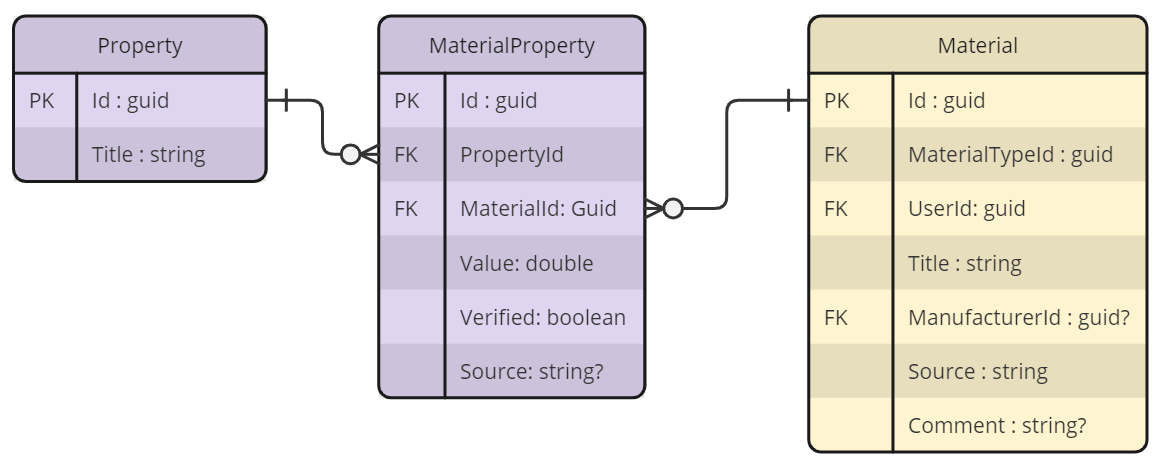
\includegraphics[width=.8\textwidth]{figures/analysis/db_desing_2.png}
    \caption[Materjali omaduste mudel]{\textit{Materjali omaduste mudel}}
    \label{fig:db_properties_model}
\end{figure}

Muus osas on andmemudeli ülesehitus on võrdlemisi lihtne. Andmemudeli diagramm tervikuna on esitatud käesoleva töö Lisas X.
Diagrammil puudub kasutaja, kasutajarollidega ja autentimisega seotud andmebaasi osa, kuna valitud raamistik (.NET) haldab
seda ise.